
% \vspace{-1mm}
\section{Introduction}

\begin{figure}[h]
    \centering
    \vspace{-4mm}
    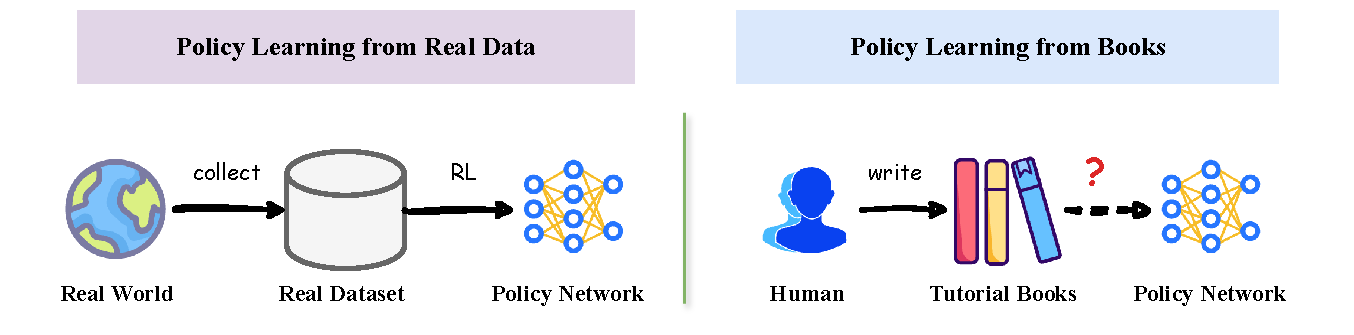
\includegraphics[width=1.0\linewidth]{fig/PER-problem.pdf}
    \caption{Comparison of the workflow of policy learning from books compared with learning from data.}
    \label{fig:problem}
    \vspace{-2mm}
\end{figure}

Humans can acquire new skills through various written materials which provide condensed knowledge, without the need of direct interactions with the target environment. 
In contrast, traditional policy learning paradigms, such as reinforcement learning (RL)~\citep{rl@2018sutton} primarily relies on trial and error~\citep{dqn2016van, ppo2017schulman, fusion2022jonas}. 
Despite recent advances in offline RL~\citep{cql@2020aviral,mopo@2020tianhe} showing that policy improvements can be achieved simply by using pre-collected data, the data collection process of the dataset can still be costly and sometimes impossible. Therefore, a question arises: similar to how humans learn, can a policy learn from books?



We argue that the recent successes of Large Language Models (LLMs) in utilizing textual data, such as GPT-4~\citep{gpt42023achiam}, and LLaMA~\citep{llama2023hugo} already demonstrated the potential to learn from textual content. However, current studies focus mainly on using LLM directly for decision making~\citep{voyager2023guanzhi, szot2023large} or integrating them as supplementary modules in other machine learning workflows~\cite{xi2023rise, hu2024survey, guo2024large}.
In this study, we introduce a novel topic built upon the shoulders of LLMs' systems: Policy Learning from Books (\topic). \topic~aims to derive a policy network directly from natural language texts, bypassing the need for numerous real-world interaction data, as shown in Figure.~\ref{fig:problem}. \textit{This can be viewed as a further step towards enabling more resources for policy learning and also a more generalized form of offline RL, which uses textbooks to learn a policy offline.} 
The essential challenge of \topic~comes from the inevitable large modality gaps between the text space, which includes the knowledge related to decision-making, and the policy network space, which formulates the parameters of the policy function. 


\begin{figure*}[h]
    \centering
    % \vspace{-5mm}
    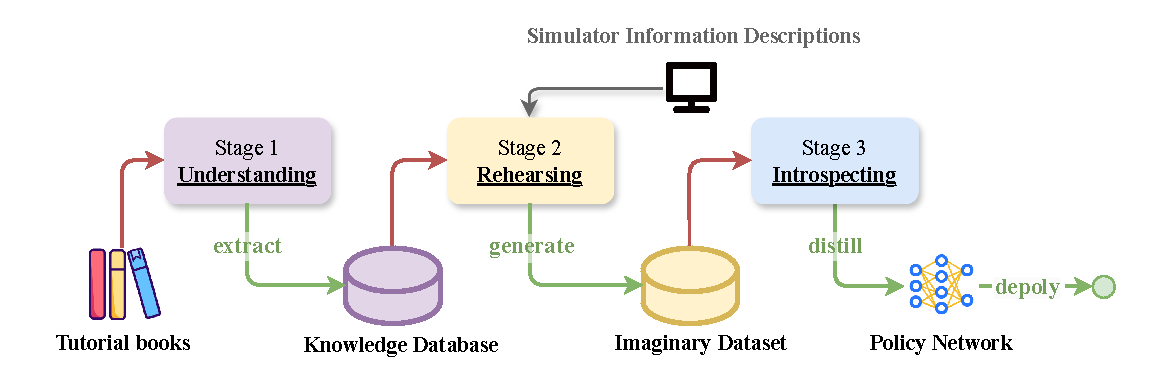
\includegraphics[width=\linewidth]{fig/framework_new.drawio (1).pdf}
    \caption{The Illustration of the understanding, rehearsal and introspection pipeline for \topic.}
    % \vspace{-2mm}
    \label{fig:framework}
\end{figure*}

To realize~\topic, inspired by human learning processes, we propose a three-stage learning methodology: understanding, rehearsal, and introspection (\algo), which is shown in Figure.~\ref{fig:framework}.  
For understanding, it first extracts knowledge from books to form a knowledge database; then it rehearses imaginary decision-making trajectories with the help of the knowledge retrieved from the database; finally, it introspects on the imaginary dataset to distill a policy network for decision-making.
We present the first practical implementation of \algo, employing LLMs to convert book paragraphs into pseudocode for policy, dynamics, and reward functions. 
This pseudocode forms a code-based knowledge database, which is used to generate an imaginary dataset based on retrieval augmented generation techniques~\citep{rag@2020patick}. A policy learning technique inspired by offline RL~\citep{mopo@2020tianhe} is then applied to distill a policy network that addresses inaccuracies in the imagined actions, rewards, and states.


% Based on the framework, we give a practical implementation for \topic: 
% It utilizes LLMs to translate paragraphs in books to pseudocode of policy function, dynamics function, and reward function respectively and form a code-based knowledge database, then generate an imaginary dataset by interactively querying an imaginary policy function, dynamics function, and reward function, which are constructed via retrieval augmented generation techniques~\citep{} with the code-based knowledge database. Finally, it uses an offline-RL-style technique for self-improving a policy network, which handles the imprecision of action, rewards, and states of the imaginary dataset together.

In the experiment, we build a testbed based on football tasks, which is popular in recent studies~\citep{football-deepmind} as a difficult decision-making task, and focus on policy learning from football tutorial books, which naturally contain condensed knowledge, especially information closely related to football skill acquisition, the environment and dynamics of football games, and ways to evaluate football behaviours. 
We collect football tutorial books from RedPajama~\citep{redpajama@2023together} and test our solution in the Google Football simulator~\citep{football2019karol}. The policy is deployed in a football game directly. Our agent controlled by the policy network could beat the built-in AI with a 37\% winning rate on average while using GPT as the football agent can only achieve a 6\% winning rate.

% The contribution of this paper can be summarized into the following three-folds. Firstly, We introduce Policy Learning from Books (\topic), a novel research idea in reinforcement learning that utilizes natural-language texts for policy learning, moving beyond the traditional reliance on real-world interaction data. Secondly, We establish a three-stage framework of \topic which mirrors human learning processes: Understanding, Rehearsing, and Introspecting (URI). URI framework represents a practical methodology of how policy can be distilled from text materials. Thirdly, we present the first practical implementation of \algo~for knowledge extraction, trajectory rehearsing, and policy distilling, based on recent advancements of LLMs, RAG, and offlineRL; We build a testbed on the football game and demonstrate the practical effectiveness and applicability of the \algo~implementation.

 %Introduction of the novel Policy Learning via Reading (\topic) approach, which uses natural-language texts for policy learning, marking a significant shift from traditional RL methods that rely heavily on real-world interaction data.